{\descr{Дослідити функцію на неперервність}}

$$
y=3^{\dfrac{2x}{3x+1}}
$$

Дослідимо функцію в точкі $-\dfrac{1}{3}$ де вона можливо має точку розриву.


$$
  \lim_{x \to -1/3 -0} 3^{\dfrac{2x}{3x+1}} \qquad \lim_{x \to (-1/3-0.001) -0} 3^{\dfrac{2x}{3x+1}} = \infty
$$

$$
  \lim_{x \to -1/3 +0} 3^{\dfrac{2x}{3x+1}} \qquad \lim_{x \to (-1/3+0.001) +0} 3^{\dfrac{2x}{3x+1}} = \infty
$$

\textbf{Висновок} - функція в точкі $-\dfrac{1}{3}$ тосить характер розриву \textbf{другого роду}, оскільки границі функції зліва та зправа прямують у нескінченність.


\begin{figure}[h!]
  \centering
  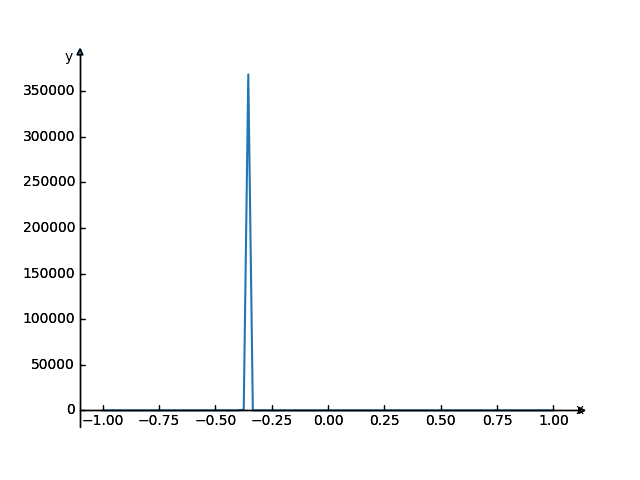
\includegraphics[width=14cm]{rozrahunkova_01/04_02.png}
  \caption{Графік функції}
  \label{fig:rr_01_40_02}
  \centering
\end{figure}
